The matrix method relates the number of events containing prompt or FNP leptons 
to the number of observed events with tight or loose-not-tight leptons 
using the probability for loose prompt or FNP leptons to satisfy the tight criteria.
The formalism for this method has been discussed in Section~\ref{sec:fake.mxm}.
The next sections will concentrate on the measurement of the 
two input variables needed for the matrix method:
the probability for loose FNP leptons to satisfy the tight selection
criteria ($\zeta$) and 
the probability for loose prompt leptons to satisfy the tight selection 
criteria ($\varepsilon$).

\subsection*{Baseline-to-signal efficiency for fake muons}

Baseline-to-signal efficiency for fake leptons (further called ``fake rate'', ($\zeta$)) is measured 
in a sample enriched in fake leptons from \ttbar\ processes.
The MC simulations indicate that this background has the largest contribution to FNP lepton background in the signal regions, 
even those with $b$-jet vetoes, due to the requirements on jet multiplicity and \met. 
The events used for the measurements require exactly two same-sign muons (and no extra baseline lepton), 
at least one $b$-jet, and at least 3 jets that were acquired by di-muon triggers.
One of the muons in the event (referred to as ``tag'') is required to satisfy signal requirements, verify $\pt>25~\GeV$, 
and trigger the event recording. 
The measurement may then be performed on the other lepton (``probe''), likely to be the fake lepton of the pair. 

%%
\begin{figure}[htb!]
\centering
\begin{tabular}{rr}
\begin{subfigure}[t]{0.5\textwidth}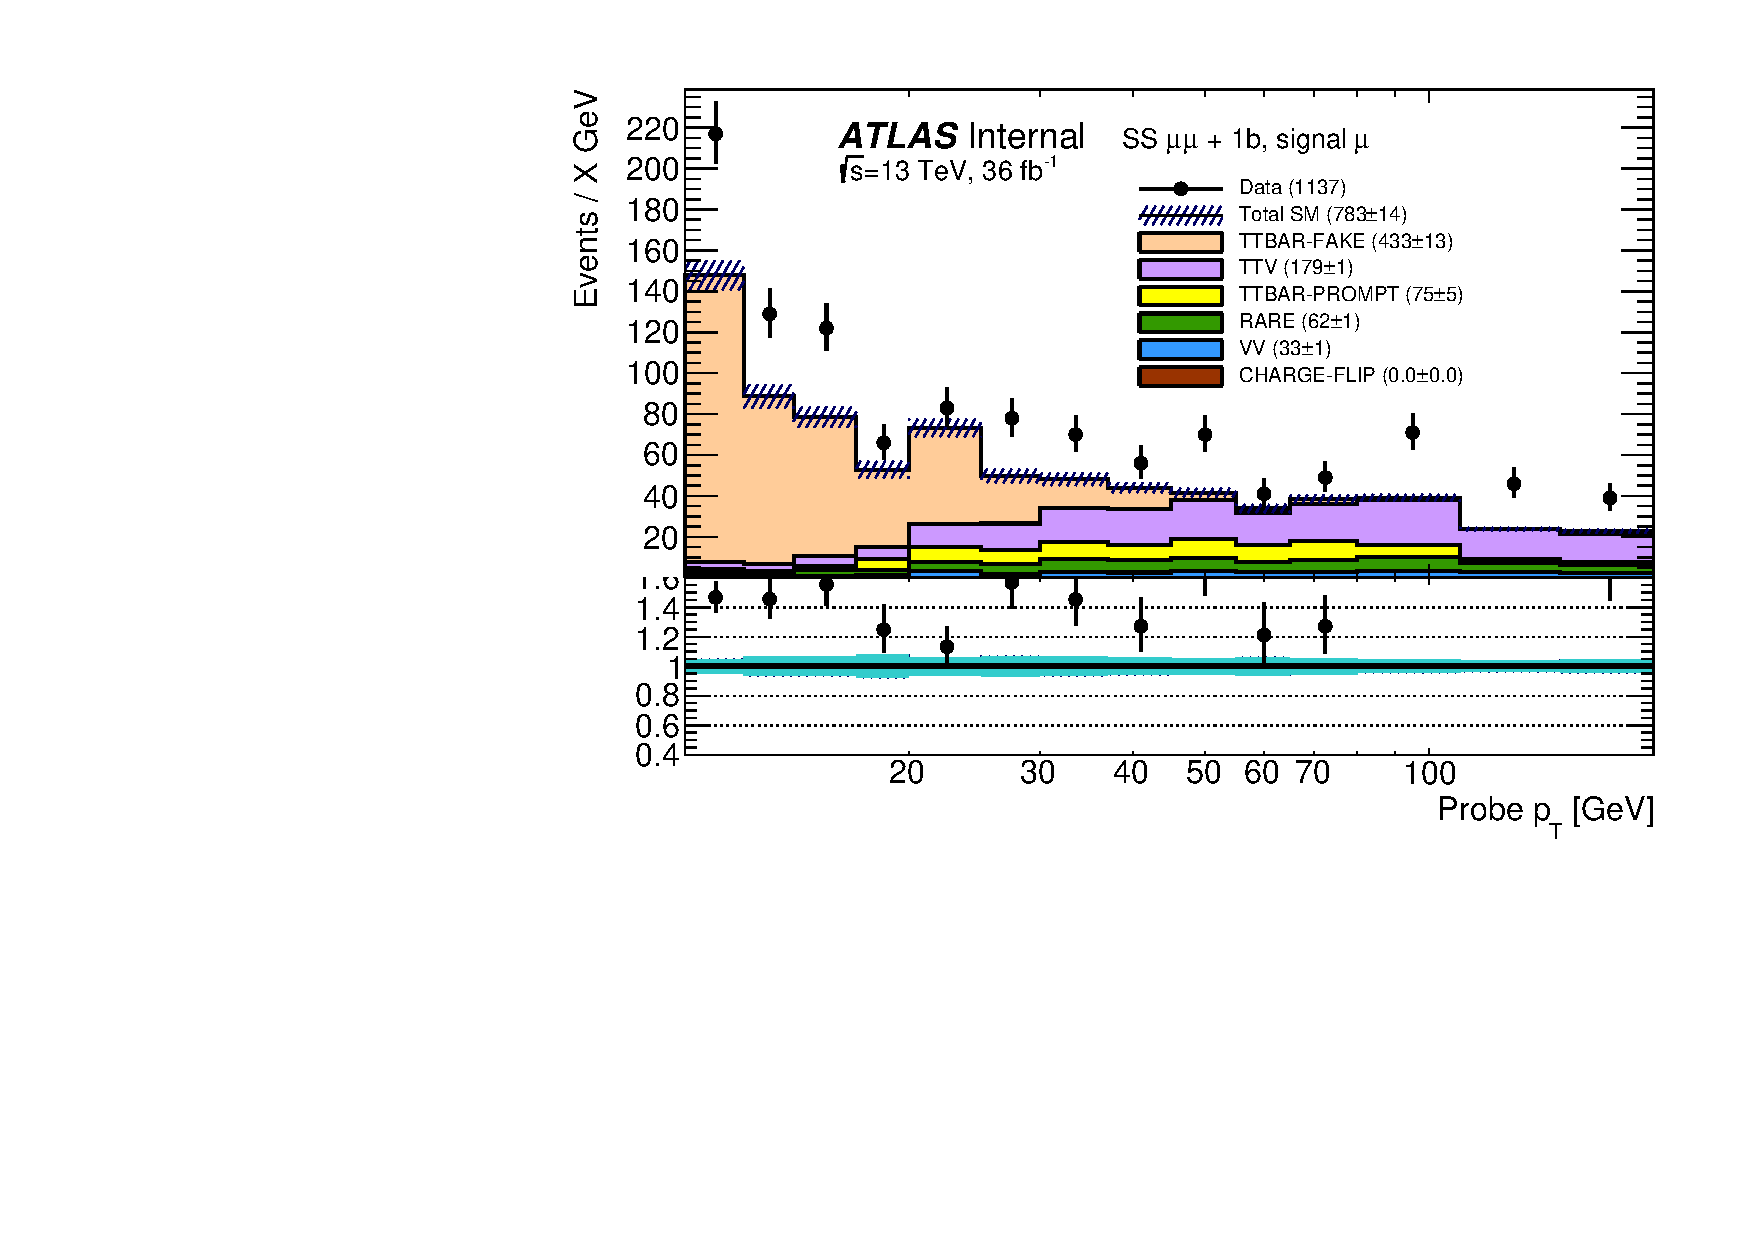
\includegraphics[width=\textwidth]{INCLUSIVETAG_PROBE_PT_MUON_SIGNAL}\caption{}\label{fig:bkg.mxm.INCLUSIVETAG_PROBE_PT_MUON_SIGNAL}\end{subfigure}&
\begin{subfigure}[t]{0.5\textwidth}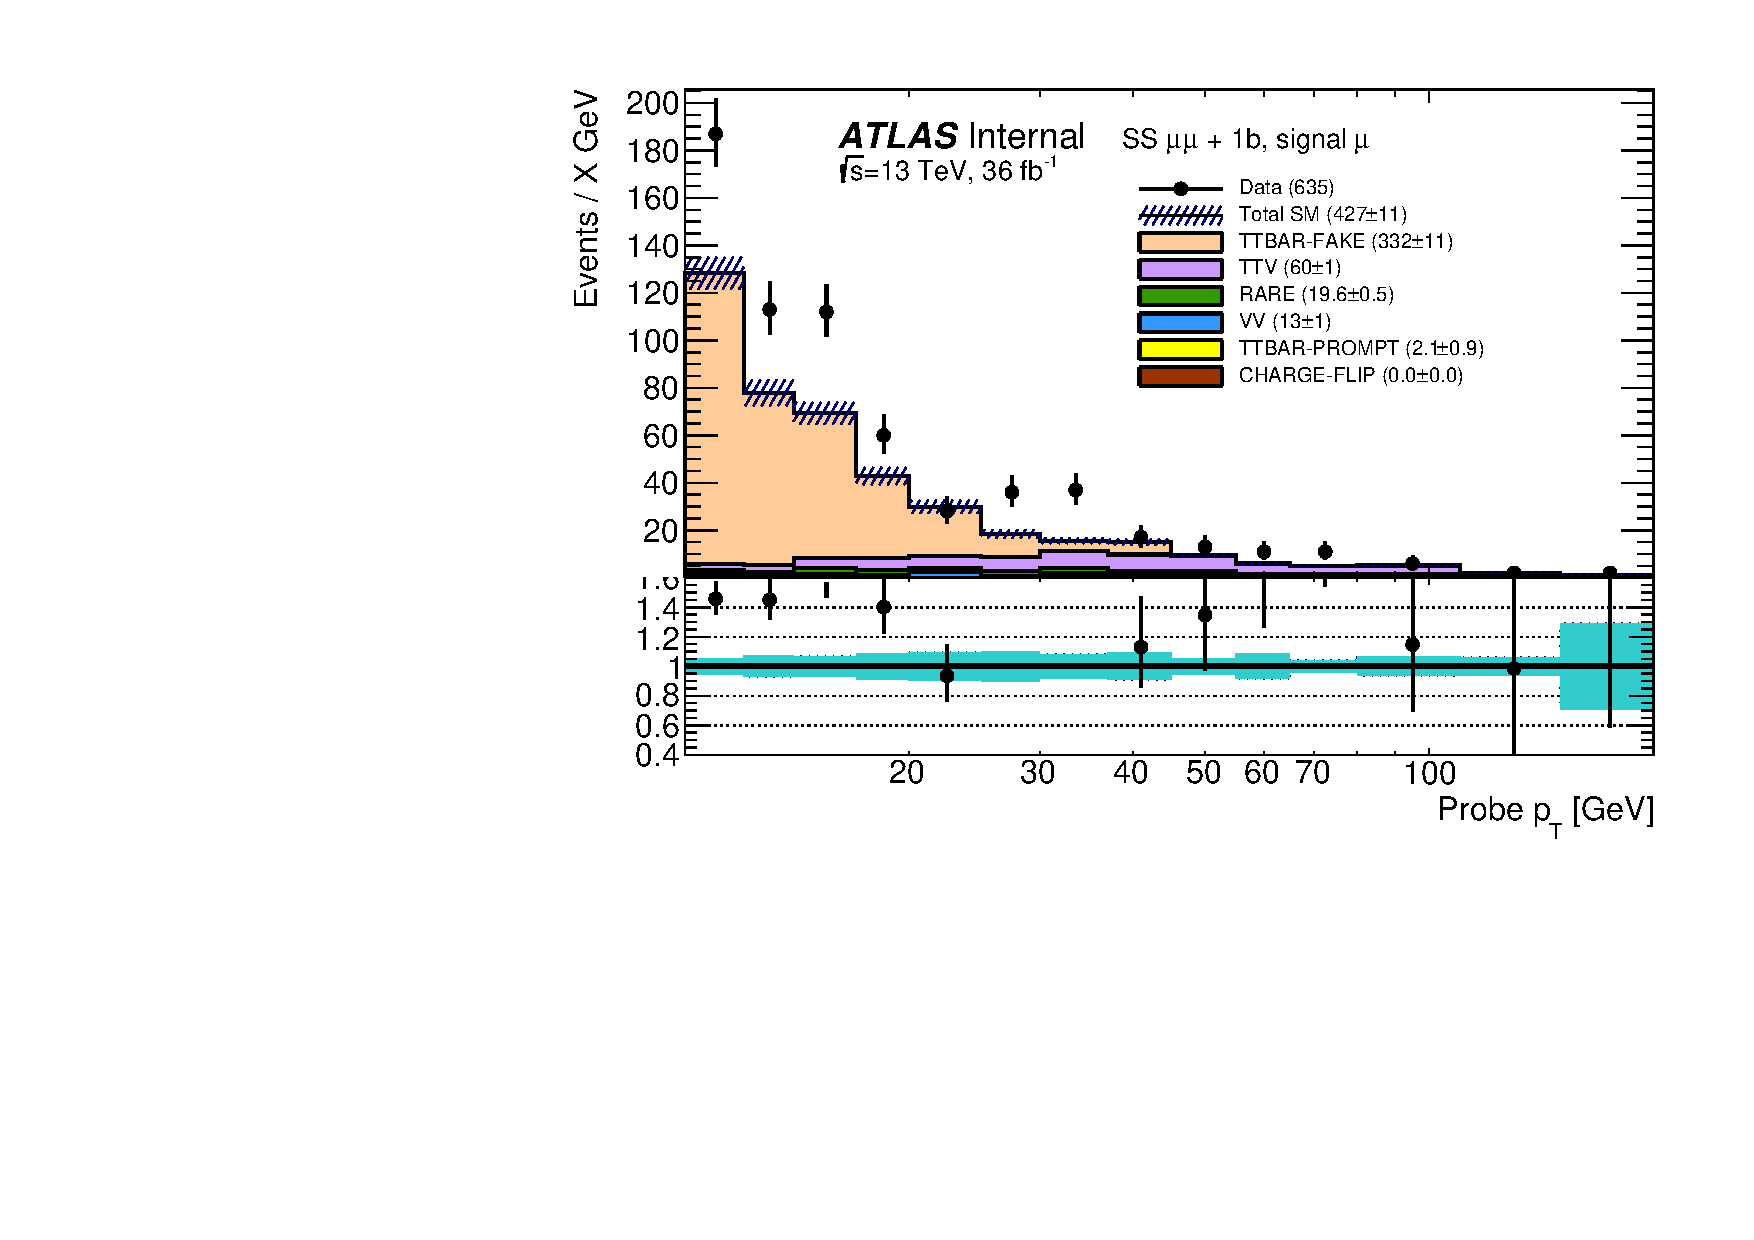
\includegraphics[width=\textwidth]{IDEALTAG_PROBE_PT_MUON_SIGNAL}\caption{}\label{fig:bkg.mxm.IDEALTAG_PROBE_PT_MUON_SIGNAL}\end{subfigure} \\
\end{tabular}
\caption
{Signal probe muon \pt\ distribution in data and MC, after pre-selection (left) 
or further tightening of the tag muon requirements (right).
The yellow area indicates $t\bar t$ events in which the tag muon is fake and the probe real, 
leading to a measurement bias. 
}
\label{Figurefakes_preselection_muon}
\end{figure}
%%

Figure~\ref{fig:bkg.mxm.INCLUSIVETAG_PROBE_PT_MUON_SIGNAL} shows the number of signal muon probes available after this pre-selection. 
It is clear that at this stage, measurements above 25 \GeV~would be very affected by the important fraction of events 
in which the tag muon is fake and the probe muon is real. 
To overcome this issue, two alternatives are considered: 
\begin{itemize}
\item tighten the \pt\ and isolation requirements of the tag muon beyond the ``signal'' requirements,
to reduce its probability of being a fake muon
\item use an identical selection for tag and probe muons, and require them to be in the same (\pt,$\eta$) bin for the measurement; 
after subtraction of estimated contributions from processes with two prompt muons, all events have one real and one fake muon, 
and the symmetry in the muon selection can be taken advantage of to obtain an unbiased measurement of the fake rate: 
$$
\zeta = \frac{\varepsilon n_2}{\varepsilon n_1+(2\varepsilon-1)n_2}
$$
%\text{ with }n_1, n_2\text{ the number of events with 1 or 2 signal muons}, 
%\text{ and }\varepsilon\text{ the efficiency for prompt muons.}
with $n_1, n_2$ the number of events with 1 or 2 signal muons, 
and $\varepsilon$ the efficiency for prompt muons.

This method is limited to measurements in inclusive or wide bins. 
It also cannot be used at too low \pt, due to contributions from processes with two fake muons (e.g. from $B\bar B$ meson production). 
\end{itemize}
Comparisons made with $t\bar t$ MC indicated that when using a very tight isolation requirement on the tag muon 
($\operatorname{max}(E_\mathrm{T}^\text{topo, cone 40},p_\mathrm{T}^\text{cone 40})<0.02\times\pt$), 
the level of bias is always largely inferior to the statistical uncertainty in the measurement, 
which itself is smaller than for the other two methods. 

Figure~\ref{fig:bkg.mxm.IDEALTAG_PROBE_PT_MUON_SIGNAL} shows the number of signal muon probes when applying those reinforced isolation criteria to the tag muon, 
as well as requiring $p_\mathrm{T}^\text{tag}>\operatorname{max}(40,p_\mathrm{T}^\text{probe}+10)$~\GeV. 
As expected, the number of pairs with a fake tag muons is down to a minor level, at least according to the simulation. 

%%
\begin{figure}[htb!]
\centering
\begin{tabular}{rr}
\begin{subfigure}[t]{0.5\textwidth}\includegraphics[width=\textwidth]{{TTBAR.Incl.FakeRate.Muon}.pdf}\caption{}\label{fig:TTBAR.Incl.FakeRate.Muon}\end{subfigure}&
\begin{subfigure}[t]{0.5\textwidth}\includegraphics[width=\textwidth]{{TTBAR.Incl.FakeRateVsEta.Muon}.pdf}\caption{}\label{fig:TTBAR.Incl.FakeRateVsEta.Muon}\end{subfigure} \\
\end{tabular}
\caption
{
Muon fake rates in $t\bar t$ MC with an inclusive selection, 
as a function of \pt\ (left, green markers) or $|\eta|$ in different momentum ranges (right). 
}
\label{Figurefakes_MC_inclusive_rates_muon}
\end{figure}
%%

Muon fake rates as predicted by the simulation ($t\bar t$, inclusive selection of leptons via truth-matching) 
are shown on Figure~\ref{Figurefakes_MC_inclusive_rates_muon} as function of \pt\ and $|\eta|$. 
One can expect a moderate dependency of the fake rates to the transverse momentum, with the strongest evolution at low \pt and a slight increase toward higher \pt. 
The fake rates are also essentially independent of the pseudorapidity, 
except at the edge ($|\eta|>2.3$) where there is a strongly pronounced increase of the rates. 
This motivates measurements in data as function of \pt\ in two $|\eta|$ bins. 

Observations in data seem to indicate that the rejection of fake tag muons by the reinforced isolation criteria 
is less important than in the simulation, or that the amount of fake muons at high \pt\ is larger than in the simulation, or both. 
This leads to an unknown level of bias in measurements performed with the straightforward tag-and-probe selection at high \pt. 
For that reason, the final rates measured in data are provided by the tag-and-probe method below 25~\GeV, 
and by the symmetric selection for $\pt>25~\GeV$. The former are obtained with 

\begin{align}
\zeta&=\frac{n_\text{signal}^\text{data} - n_\text{signal}^\text{MC}}{n_\text{baseline}^\text{data} - n_\text{baseline}^\text{MC}}\\
\text{with }&\Delta\zeta_\text{stat} = \frac{\sqrt{(1-2\zeta)n_\text{signal}^\text{data} + \zeta^2 n_\text{baseline}^\text{data}}}
{n_\text{baseline}^\text{data} - n_\text{baseline}^\text{MC}}\notag
%\text{and }&\Delta\zeta_\text{syst} = \frac{\Delta B}{B}\times\frac{\sqrt{(1-\zeta^2)(n_\text{signal}^\text{MC})^2 
%+ \zeta^2 (n_\text{baseline}^\text{MC} - n_\text{signal}^\text{MC})^2 }}
\end{align}
while the latter are obtained with:
\begin{align}
\zeta &= \frac{\varepsilon (n_\text{both signal}^\text{data} - n_\text{both signal}^\text{MC})}
{\varepsilon (n_\text{only 1 signal}^\text{data} - n_\text{only 1 signal}^\text{MC})
+(2\varepsilon-1)(n_\text{both signal}^\text{data} - n_\text{both signal}^\text{MC})}\\
\text{with }&\Delta\zeta_\text{stat} 
= \frac{\zeta}{n_\text{both signal}^\text{data} - n_\text{both signal}^\text{MC}}
\sqrt{\zeta^2 n_\text{only 1 signal} + \left(1-\frac{2\varepsilon-1}{\varepsilon}\zeta\right)^2 n_\text{both signal}}.\notag
\end{align}
The efficiency for prompt muons $\varepsilon$ is assigned values compatible with section~\ref{subsubsec:fakes_matrix_real_efficiency}. 

The measured rates are presented in Table~\ref{table:fake_rates_muon}. 
The central values are shown together with the associated statistical uncertainty, 
as well as the propagation of the uncertainty on the subtracted backgrounds normalization, 
which is taken as a global $\Delta B/B=20\%$. 
The rates are of the order of $10\%$ up to 30 \GeV, beyond which they increase. 
Overall these values are not very different from those predicted by the simulation. 

%%
\begin{table}[htb!]
\def\arraystretch{1.15}
\def\arraystretch{1.15}
\centering
\resizebox{\textwidth}{!}{
\begin{tabular}{|c|c|c|c|} \hline\hline
\multicolumn{2}{|c|}{$10<\pt<12~\GeV$}         & \multicolumn{2}{c|}{$12<\pt<14$}                  \\  
\hline 
$|\eta|<2.3$             & $|\eta|>2.3$             & $|\eta|<2.3$             & $|\eta|>2.3$            \\
\hline
$0.14 \pm 0.01 \pm 0.00$ & $0.22 \pm 0.05 \pm 0.00$ & $0.11 \pm 0.01 \pm 0.00$ & $0.24 \pm 0.06 \pm 0.00$ \\ 
\hline
\end{tabular}}

\resizebox{\textwidth}{!}{
\begin{tabular}{|c|c|c|c|} \hline
\multicolumn{2}{|c|}{$14<\pt<17$}                    & \multicolumn{2}{c|}{$17<\pt< 20~\GeV$}       \\       
\hline
$|\eta|<2.3$             & $|\eta|>2.3$             & $|\eta|<2.3$             & $|\eta|>2.3$            \\    
\hline
$0.12 \pm 0.01 \pm 0.00$ & $0.09 \pm 0.05 \pm 0.00$ & $0.09 \pm 0.01 \pm 0.00$ & $0.21 \pm 0.07 \pm 0.00$ \\
\hline 
\end{tabular}}

\resizebox{\textwidth}{!}{
\begin{tabular}{|c|c|c|c|c|} \hline
             $20<\pt<30$ &              $30<\pt<40$ &              $40<\pt<60$ &                $\pt>60$ \\
\hline
$0.07 \pm 0.02 \pm 0.00$ & $0.12 \pm 0.05 \pm 0.01$ & $0.16 \pm 0.09 \pm 0.04$ & $0.49 \pm 0.10 \pm 0.07$ \\
\hline \hline
\end{tabular}}
\caption{Muon fake rate measured in data and the associated statistical uncertainty. 
The systematic uncertainty originating from the subtraction of ``backgrounds'' with only prompt leptons is also displayed. }
\label{table:fake_rates_muon}
\end{table}

Some of the validation and signal regions require events with 2 or more $b$-tagged jets, 
which reduces the fraction of non-prompt muons coming from $B$ meson decays. 
Figure~\ref{fig:fakes_MC_vsBjets_muon} illustrates how this impacts 
the fake rates. 
Given the good agreement between data and simulation for the measured values, 
a correction is applied to the measured rates for events with $\ge 2$ $b$-jets, 
taken directly from simulated $t\bar t$ events. 
This correction factor varies between 1 and 2 with \pt, 
and the whole size of the correction is assigned as an additional systematic uncertainty (see Table~\ref{tab:fake_rates_muon_systematics}). 

\begin{table}[htb!]
\def\arraystretch{1.15}
\def\arraystretch{1.15}
\centering
\resizebox{\textwidth}{!}{
\begin{tabular}{|c|c|c|c|c|c|c|} \hline\hline
 \pt & $<14$ & $14-20$ & $20-30$ & $30-40$ & $40-60$ & $>60$\\\hline
$\Delta\zeta^\text{(syst)}$ & 30\% & 30\%  & 30\%     &  50\%   & \multicolumn{2}{c|}{
		\begin{tabular}{@{}c@{}}50\% for $H_\mathrm{T}<600$ \\ 70\% for $600<H_\mathrm{T}<1200$ \\85\% for $H_\mathrm{T}>1200$\end{tabular}} \\\hline
$\frac{\zeta_{\ge 2b}}{\zeta}$ & $1.2\pm 0.2$ & $1.5\pm 0.5$ & $1.7\pm 0.7$ & $2.0\pm 1.0$ & $1.5\pm 0.5$ & $-$\\\hline
\end{tabular}}
\caption{Additional systematic uncertainty on the muon fake rates, to address variations of the latter in different environments. 
The table also shows the correction factors and uncertainties applied to final states with $\ge 2$ $b$-tagged jets.}
\label{tab:fake_rates_muon_systematics}
\end{table}


%%
\par{\bf Systematic uncertainties\\}
To cover potential differences in the fake rates between the measurement regions and the signal regions, 
that could be due to different origins or kinematic properties of the fake leptons, 
uncertainties are set based on the extent of those differences predicted by the simulation. 
The largest effect is the decrease of the fake rates with $H_\mathrm{T}$ (especially for high-\pt\ muons), 
which likely correlates to a harder jet at the origin of the non-prompt muon, hence a reduced likelihood to satisfy isolation requirements. 
Table~\ref{tab:fake_rates_muon_systematics} summarizes the additional systematic uncertainties applied to the muon fake rates. 
They vary from $30\%$ at low \pt, to up to 85\% for $\pt>40~\GeV$; in that range, the uncertainties are made $H_\mathrm{T}$-dependent. 

As already shown, Figure~\ref{fig:fakes_MC_vsBjets_muon} shows the variation of the fake rate in $t\bar t$ MC as a function of the number of $b$-tagged jets in the event. 
Unsurprisingly, the rates are very similar for $0b$ and $\ge 1b$ final states, 
justifying the use of the fake rates measured in this section (i.e. in a $\ge 1b$ region) to predict fake muon background in all signal regions. 

\begin{figure}[htb!]
\centering
\includegraphics[width=0.49\textwidth]{{TTBAR.BjetImpact.FakeRate.Muon}.pdf}
\caption
{
Muon fake rates in $t\bar t$ MC with an inclusive selection, 
as function of \pt\ and split according to the number of $b$-tagged jets in the event. 
}
\label{fig:fakes_MC_vsBjets_muon}
\end{figure}

\subsection*{Baseline-to-signal efficiency for fake electrons}
\label{subsubsec:fakes_matrix_fake_rate_electrons}


%%
\begin{figure}[htb!]
\centering
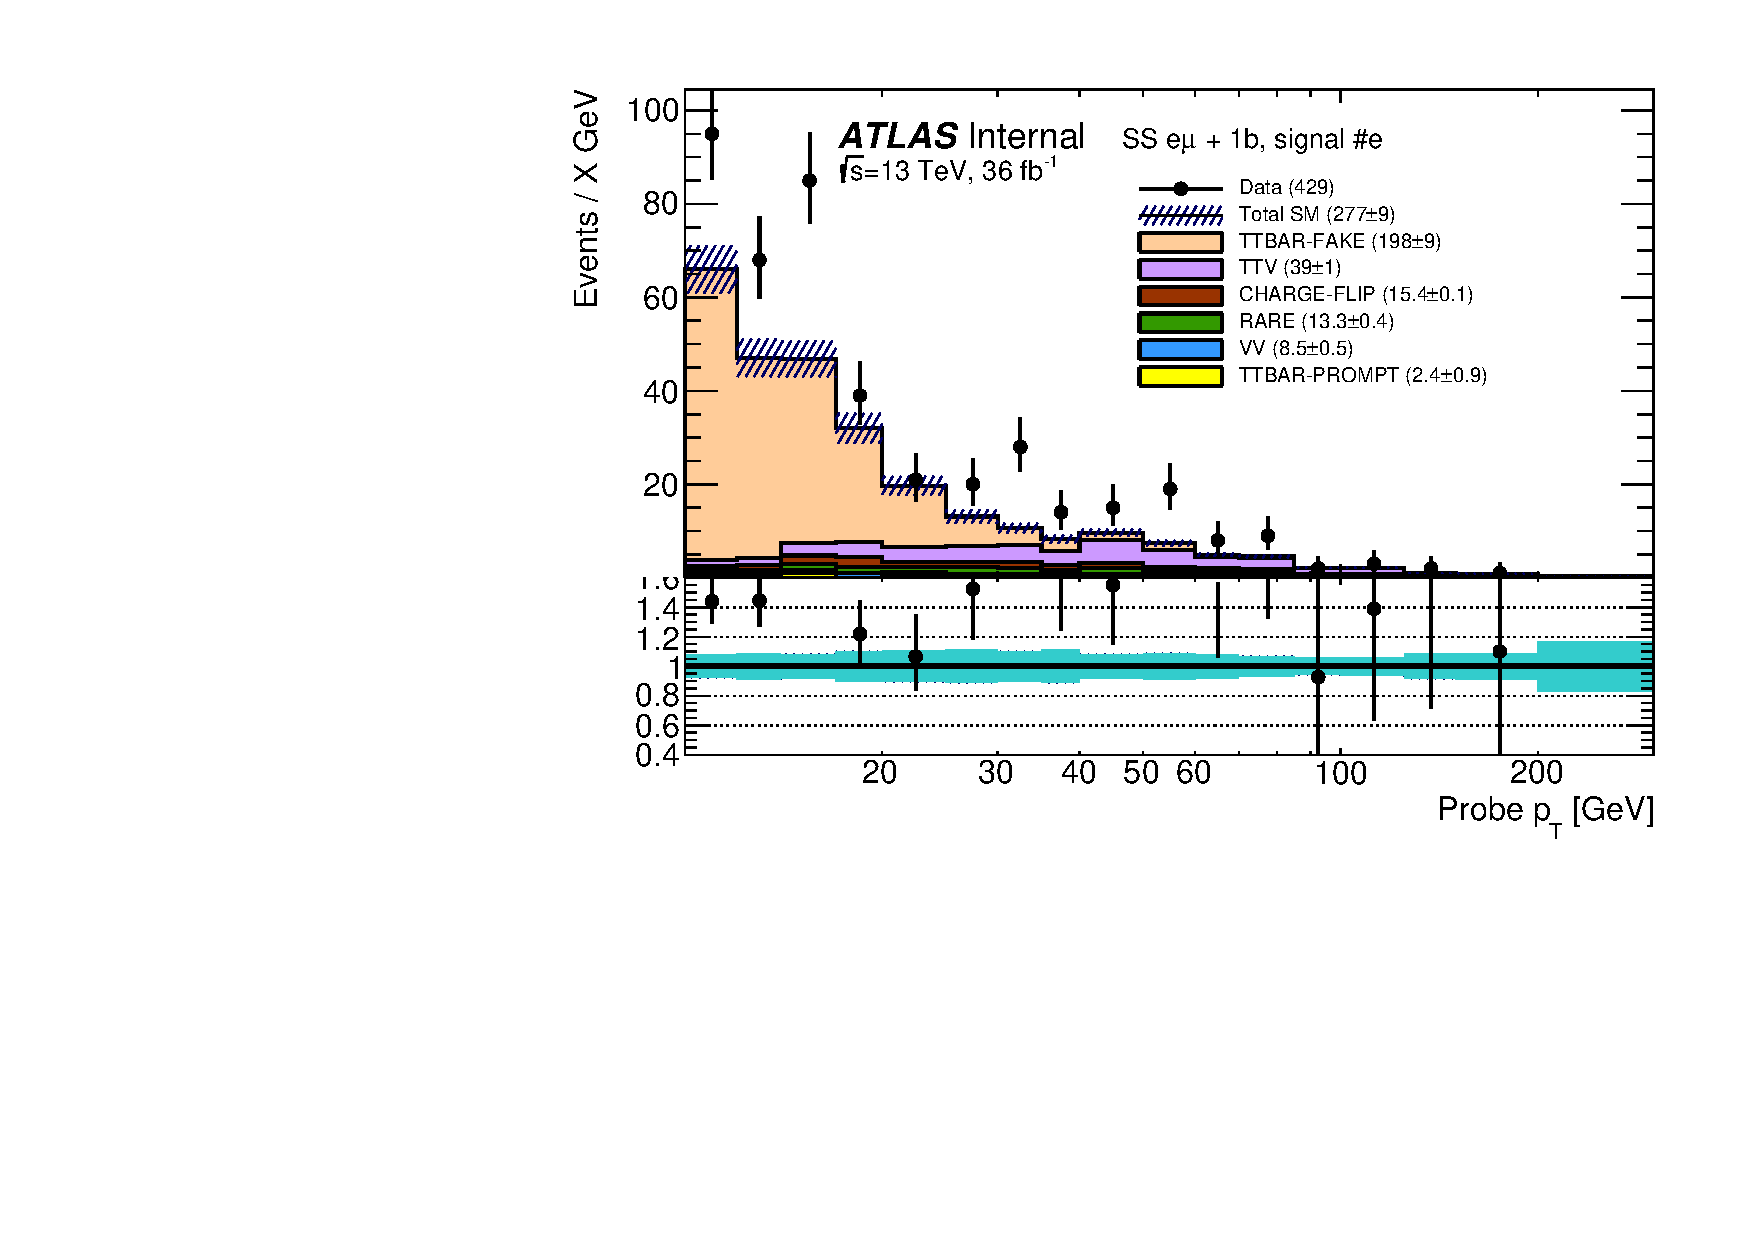
\includegraphics[width=0.49\textwidth]{IDEALTAG_CFTPROBE_PT_ELECTRON_SIGNAL}
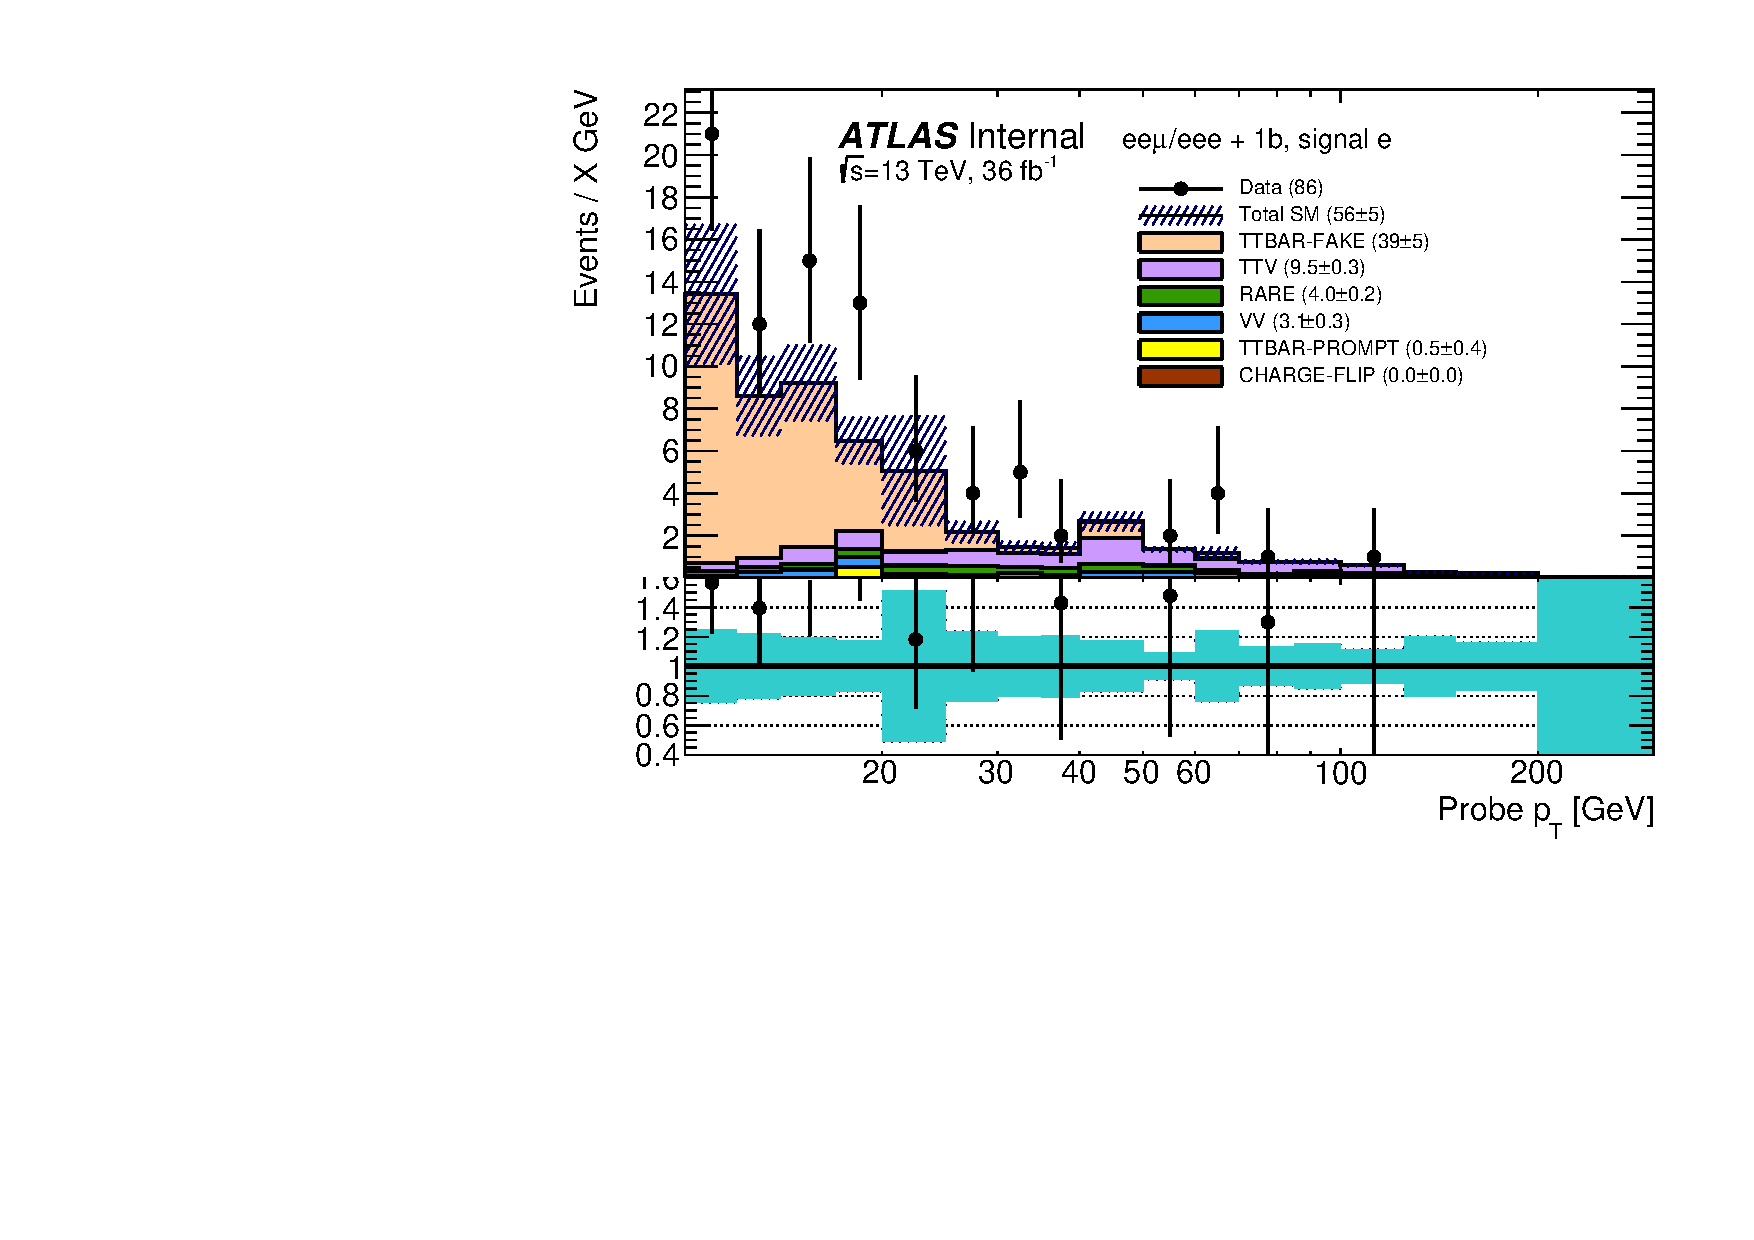
\includegraphics[width=0.49\textwidth]{TRILEP_IDEALTAG_PROBE_PT_ELECTRON_SIGNAL}
\caption
{Signal probe electron \pt\ distribution in data and MC, for $e^\pm\mu^\pm$ pairs (left, with probe electrons satisfying  a reinforced tag muon selection) 
or $\ell^\pm e^\mp e^\mp$ pairs (right, with reinforced tag electron selection), 
as described in section~\ref{subsubsec:fakes_matrix_fake_rate_electrons}. 
The yellow area indicates $t\bar t$ events in which the tag lepton is fake and the probe electron real, 
leading to a measurement bias. 
}
\label{Figurefakes_preselection_electron}
\end{figure}
%%

Electron fake rates are measured with a similar methodology, but the $e^\pm e^\pm$ channel is unusable due to the presence of a large charge-flip background. 
This is overcome by working with $e^\pm\mu^\pm$ pairs instead (with a tag muon), but mixing leptons of different flavours brings additional complications 
(for example, the unbiased measurement cannot be employed to measure muon fake rates at higher \pt, as there is no symmetry between the leptons). 
To improve confidence, measurements are performed in four different ways, which complement each other: 
\begin{itemize}
\item straightforward tag-and-probe with $e\mu$ pairs, with the same tag muon selection as in the previous section. 
\item same selection, but subtracting from the numerator the number of pairs with one fake tag muon and one prompt probe electron, 
itself estimated from the number of observed $e\mu$ events with a muon failing signal requirements, 
scaled by an efficiency correction factor $e\mu/\mu\mu$ taken from $t\bar t$ MC (only for pairs with one fake muon). 
This only works if the two muons satisfy the same kinematic requirements, therefore can be used only for measurements in wide or inclusive bins. 
\item selecting $\ell^\mp e^\pm e^\pm+\ge 1b$ events, with a $Z$ veto on SFOS pairs. 
This selection entirely suppresses contributions from charge-flip, or events with fake muons. 
One of the electron, with standard signal requirements, is required to satisfy the same reinforced \pt\ and isolation requirements as for the muon measurement,
and the measurement can be performed on the other electron. 
\item same selection, using the symmetry between the two same-sign electrons to measure the rates in an unbiased way, similarly to the muon case. 
\end{itemize}
Events are acquired with the combination of single-muon (as in previous section) and $e\mu$ triggers. 


Figure~\ref{Figurefakes_preselection_electron} shows the number of signal probe electrons selected in the $e\mu$ and $\ell ee$ channels. 
There are significantly fewer events selected in the trilepton channel. 
Figure~\ref{Figurefakes_MC_inclusive_rates_electron} shows the electron fake rate as a function of \pt\ or $\eta$ in $t\bar t$ MC. 
The variations of the rates as function of the pseudorapidity are not very large, 
therefore measurements are only performed as a function of \pt. 
The low \pt\ range is dominated by non-prompt electrons from heavy flavour decays, while beyond 30~\GeV, 
electron fakes mostly come from conversions of photons produced inside jets, such as $\pi^0\to\gamma\gamma$ decays. 

%%
\begin{figure}[htb!]
\centering
\includegraphics[width=0.49\textwidth]{{TTBAR.Incl.FakeRate.Electron}.pdf}
\includegraphics[width=0.49\textwidth]{{TTBAR.Incl.FakeRateVsEta.Electron}.pdf}
\caption
{
Electron fake rates in $t\bar t$ MC with an inclusive selection, 
as function of \pt\ (left, yellow/green markers = with/without CFT cut applied) or $|\eta|$ in different momentum ranges (right). 
}
\label{Figurefakes_MC_inclusive_rates_electron}
\end{figure}
%%

Based on the estimated levels of bias, and achievable statistical precision of the different methods, 
the electron fake rate is measured with the tag-and-probe $e\mu$ selection up to 30~\GeV, 
and by combining ``unbiased'' evaluations in both $e\mu$ and $\ell ee$ channels beyond. 
The measured rates are presented in Table~\ref{table:fake_rates_electron}, 
together with the associated statistical and background-subtraction uncertainties. 
The rates are of the order of $10\%$ up to 30 \GeV, beyond which they increase 
up to 25\%. 

%%
\begin{table}[htb!]
\def\arraystretch{1.15}
\def\arraystretch{1.15}
\centering
\resizebox{\textwidth}{!}{
\begin{tabular}{|c|c|c|c|} \hline\hline
             $10<\pt<12$ &              $12<\pt<14$ &              $14<\pt<17$ &             $17<\pt<20$ \\
$0.10 \pm 0.01 \pm 0.00$ & $0.10 \pm 0.01 \pm 0.01$ & $0.12 \pm 0.01 \pm 0.01$ & $0.08 \pm 0.02 \pm 0.00$ \\
\hline \hline
\end{tabular}}

\resizebox{\textwidth}{!}{
\begin{tabular}{|c|c|c|c|} \hline\hline
             $20<\pt<25$ &              $25<\pt<30$ &              $30<\pt<40$ &             $40>\pt$ \\
$0.07 \pm 0.02 \pm 0.01$ & $0.11 \pm 0.03 \pm 0.01$ & $0.20 \pm 0.07 \pm 0.03$ & $0.25 \pm 0.10 \pm 0.05$ \\
\hline \hline
\end{tabular}}
\caption{Electron fake rate measured in data and the associated statistical uncertainty. 
The systematic uncertainty originating from the subtraction of ``backgrounds'' with only prompt leptons is also displayed. }
\label{table:fake_rates_electron}
\end{table}

Unlike muons, MC-based correction factors are not applied for final states with $\ge 2$ $b$-tagged jets. 
This is because there is less good agreement between the measured rates and the simulation; 
in particular the former take larger values in the medium-\pt\ range. 
%%

\par{\bf Systematic uncertainties\\}
Similarly to the muon case, systematic uncertainties are assigned to cover for difference in the rates in the measurement regions and in the signal regions
that would be due to different sources of fake leptons, or different kinematic properties of these sources. 
Unlike muons, there is much less of a dependency to $H_\mathrm{T}$. 
The dominant source of potential differences is therefore the origin of the fake electron (see Figure~\ref{fig:fakes_MC_perSource_electron}); 
for $\pt<20~\GeV$, non-prompt electrons from heavy--flavor hadron decays dominate,
which is confirmed by the good agreement between MC fake rates and those measured in data. 
In that range, an uncertainty of $30\%$ is assigned to the fake rates (inflated to $50\%$ for final states with $\ge 2b$-tagged jets). 
The rates measured in data are larger than those predicted by the simulation, 
and would for example be consistent with a larger amount of electrons from photon conversions than predicted. 
In that range, an uncertainty of $50\%$ is assigned to cover any arbitrary variation of the relative contributions of each source. 

Finally, Figure~\ref{fig:fakes_MC_perSource_electron} shows the variation of the fake rate in $t\bar t$ MC as function of the number of $b$-tagged jets in the event. 
As expected, the rates are very similar for $0b$ and $\ge 1b$ final states, 
justifying the use of the fake rates measured in this section (i.e. in a $\ge 1b$ region) to predict fake electron background in all signal regions. 
%We do not assign extra uncertainties for final states with $\ge 2b$-jets for $\pt>20$ GeV: if, indeed, the relative contribution of HF decays is smaller than expected in that range, 
%then there should be less intrinsic difference between $0/1b$ and $\ge 2b$ final states, and those are already within the existing uncertainties. 

\begin{figure}[htb!]
\centering
\includegraphics[width=0.49\textwidth]{{TTBAR.Incl.FakeRate.PerSource.Electron}.pdf}
\includegraphics[width=0.49\textwidth]{{TTBAR.BjetImpact.FakeRate.Electron}.pdf}
\caption
{
Electron fake rates in $t\bar t$ MC with an inclusive selection, 
as a function of \pt\ and split according to the source of the fake electron (left). 
The relative contributions of each source (for signal electrons) are indicated on the right-hand-side. 
}
\label{fig:fakes_MC_perSource_electron}
\end{figure}


\subsection*{Baseline-to-signal efficiency for real leptons}
\label{subsubsec:fakes_matrix_real_efficiency}

% mostly copy-pasted from 2015 supporting note

Baseline-to-signal efficiency for real leptons is measured in a high purity data sample of opposite-sign same-flavor leptons with the standard $Z$ tag-and-probe method.
Events are selected by a single lepton trigger.
%\texttt{e24\_lhmedium\_iloose\_L1EM20VH}  or \texttt{e26\_lhtight\_nod0\_ivarloose} for electrons,
%\texttt{mu20\_iloose\_L1MU15} or \texttt{mu26\_ivarmedium} for muons,
%respectively in 2015 or 2016 data. 
The tag lepton, required to have triggered the event recording, also satisfies signal requirements and verifies $\pt>25~\GeV$. 
The probe lepton used for the efficiency measurement satisfies baseline requirements. 
All possible tag-and-probe combinations are considered in an event (including permutation of the tag and probe leptons), 
as long as the invariant mass of the pair is comprised between 80 and 100~\GeV. 
Figure~\ref{fig:RLE_mll_distribution} illustrates this event selection.

\begin{figure}[htb!]
\centering
\begin{subfigure}[b]{0.45\textwidth}
	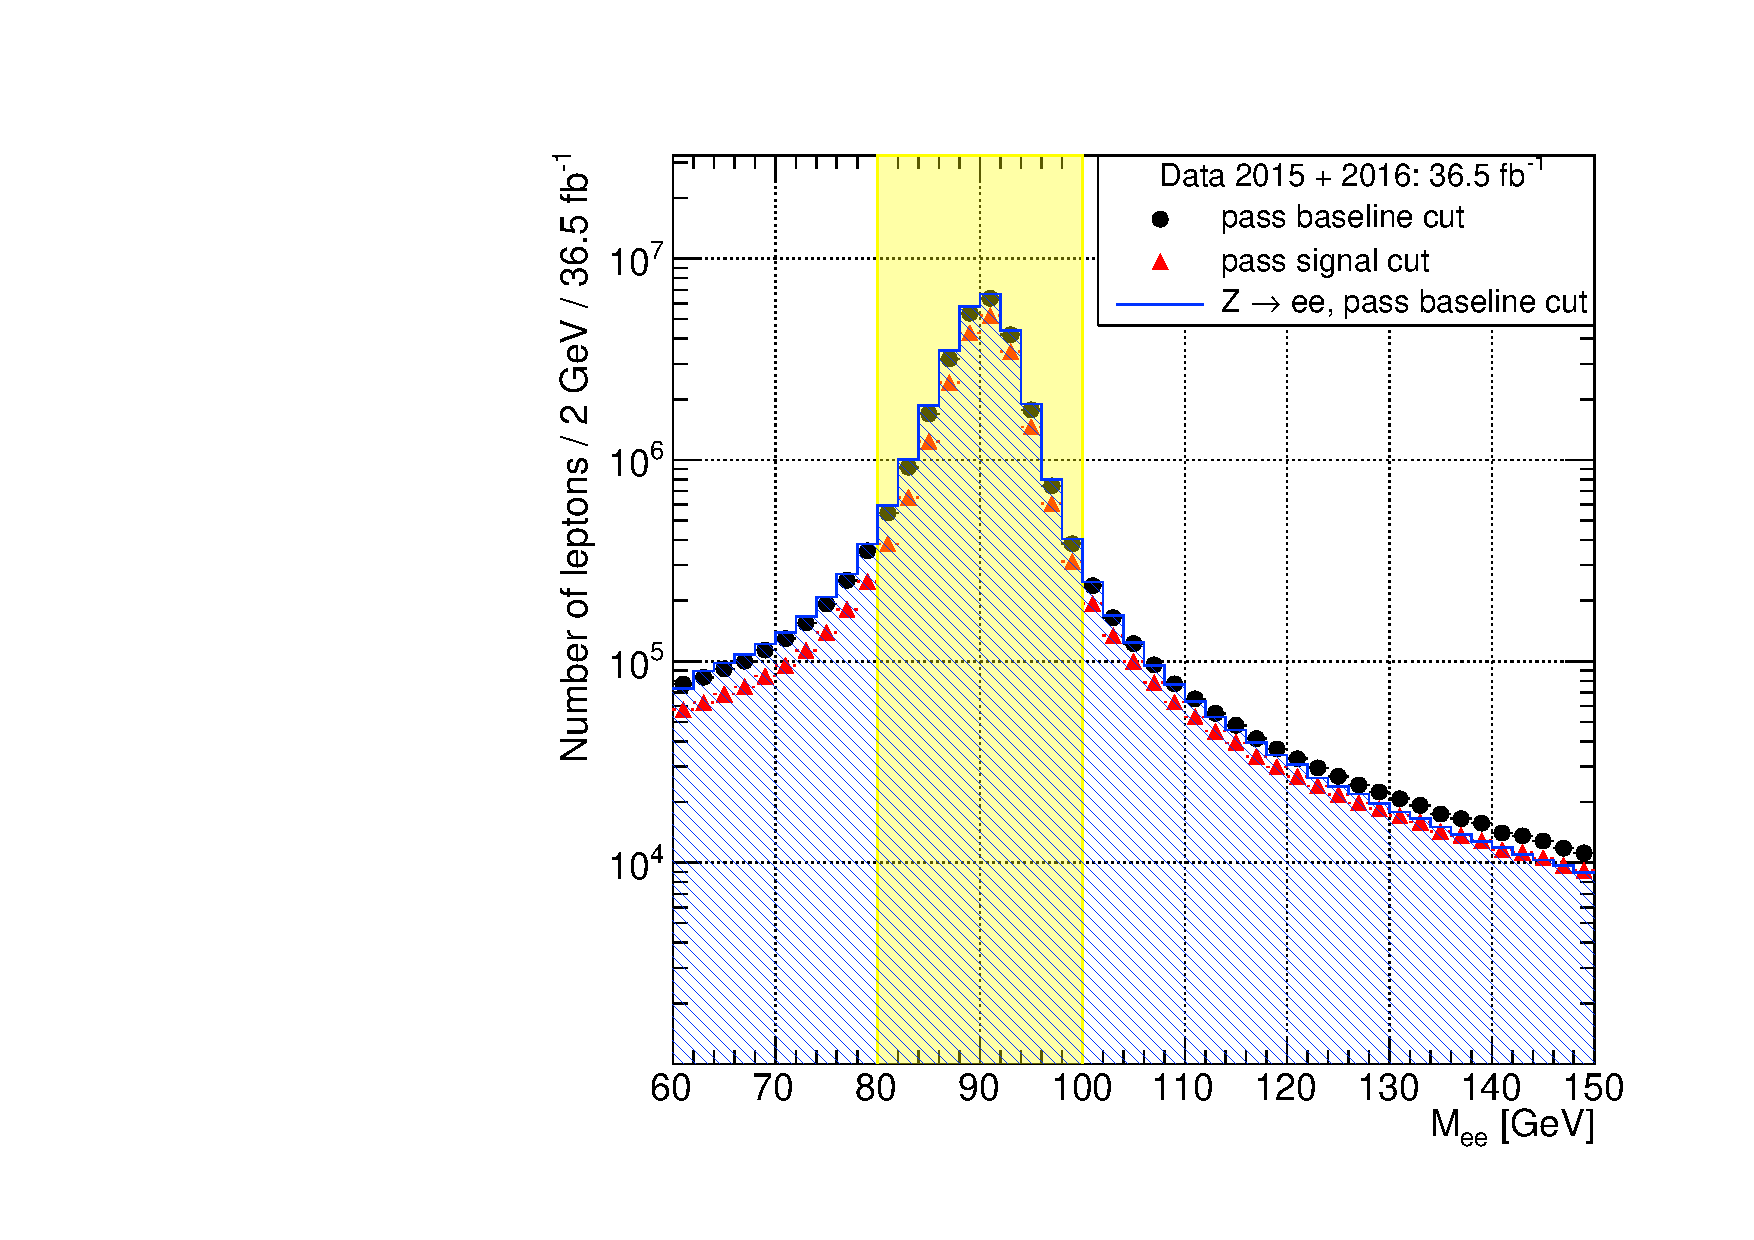
\includegraphics[width=\textwidth]{baseline_and_signal_mll_distribution_Mee.pdf}
\end{subfigure}
\begin{subfigure}[b]{0.45\textwidth}
	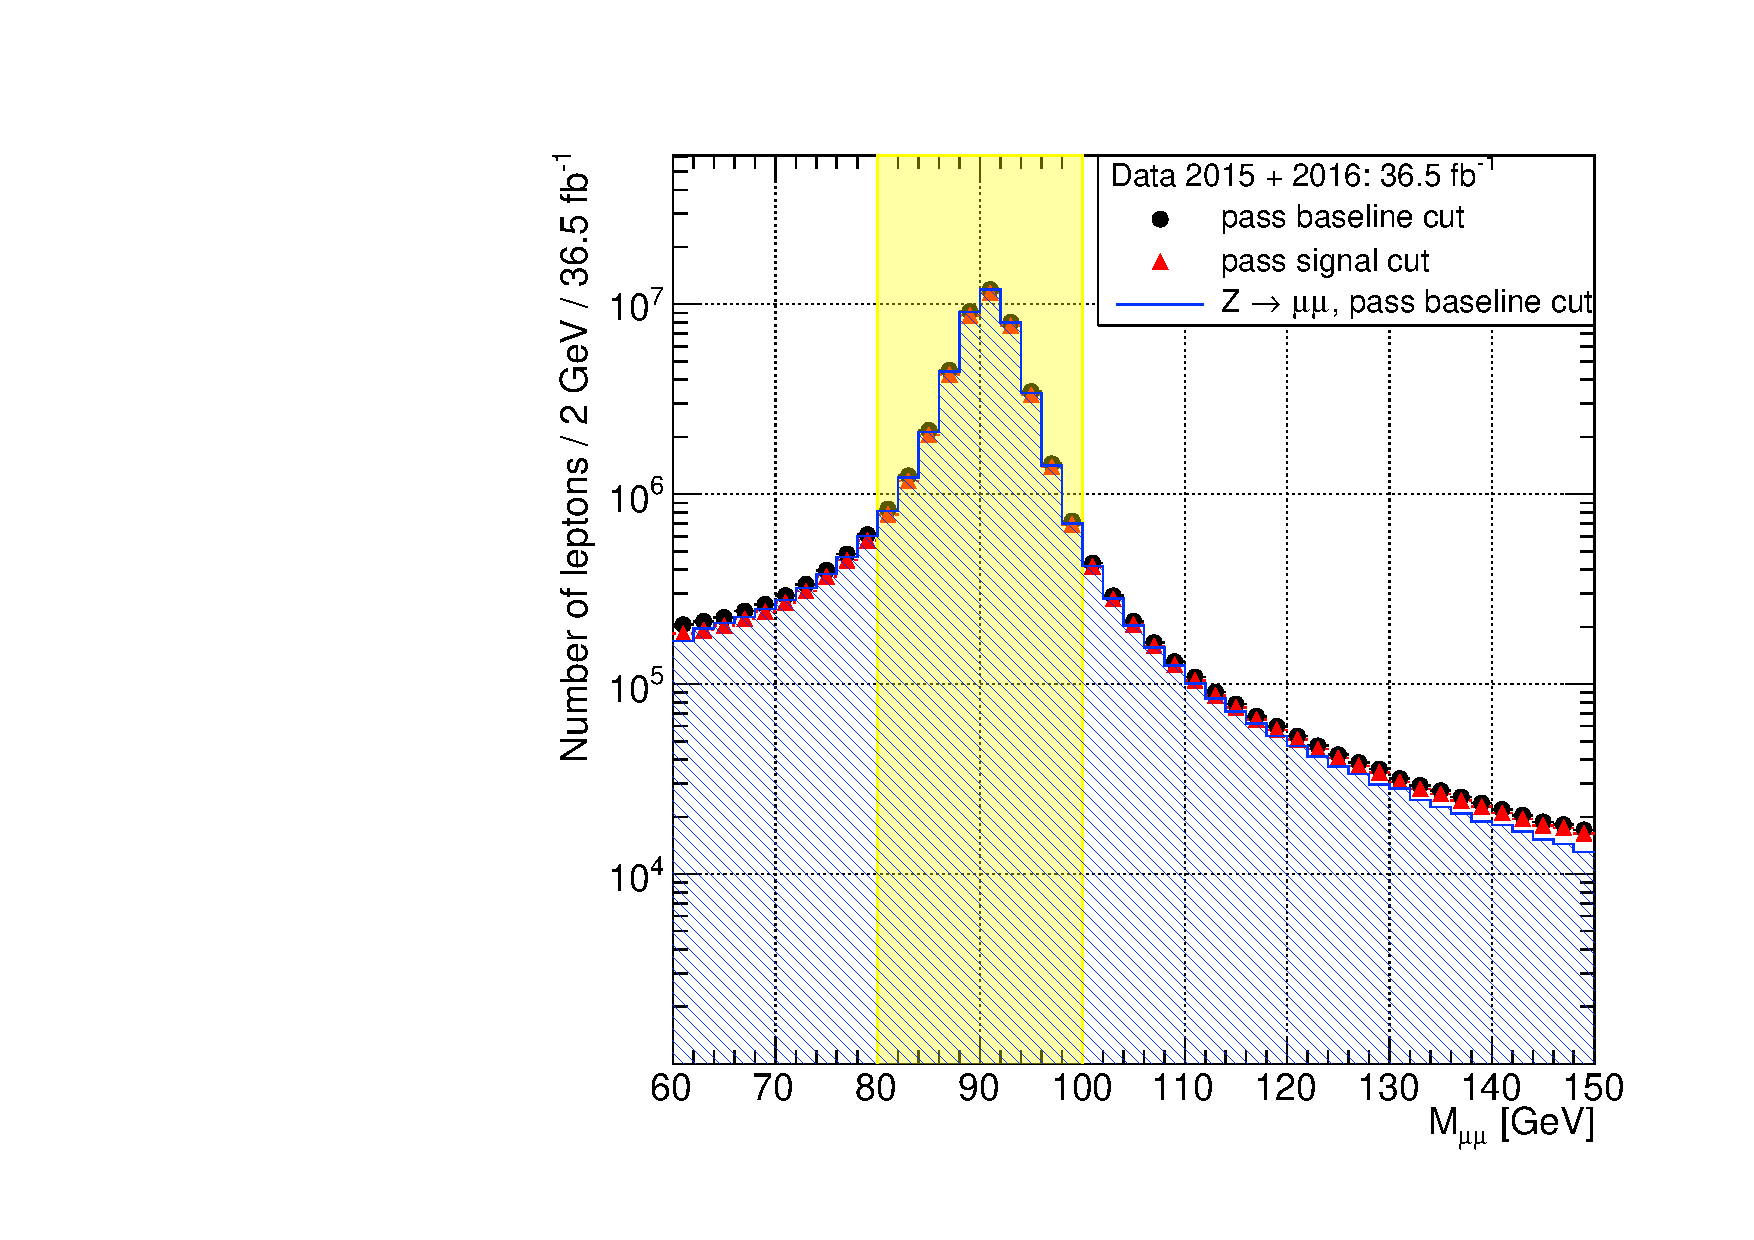
\includegraphics[width=\textwidth]{baseline_and_signal_mll_distribution_Mmumu.pdf}
\end{subfigure}
\caption{Invariant mass of opposite-sign same-flavor electrons (left) and muons (right), after the tag selection, 
where the probe satisfies the baseline requirements or the signal requirements.}
\label{fig:RLE_mll_distribution}
\end{figure}

A non-negligible background contamination in the electron channel affects measurements below $\pt=20~\GeV$. 
This contamination is taken into account in the measurement using a background template method inspired by the method used to measure reconstruction, identification, and 
isolation efficiencies documented in~\cite{ATLAS-CONF-2014-032}. 
This template is built from the tag-and-probe invariant mass distribution for baseline-level probe electrons that fail both tight identification
 and isolation requirements, smoothed by assuming an exponential shape whose parameters are determined by a fit in the interval $60<m_{ee}<120~\GeV$ excluding the $80<m_{ee}< 100~\GeV$ region. 
The background template is then normalized to the main tag-and-probe distribution in the background-dominated tail $120<m_{ee}<150~\GeV$. 
The estimated level of background goes up to $4\%$, reached for probe electrons with $\pt<15~\GeV$ and $|\eta|<0.8$. 

\begin{figure}[htb!]
\centering
\begin{subfigure}{0.49\textwidth}
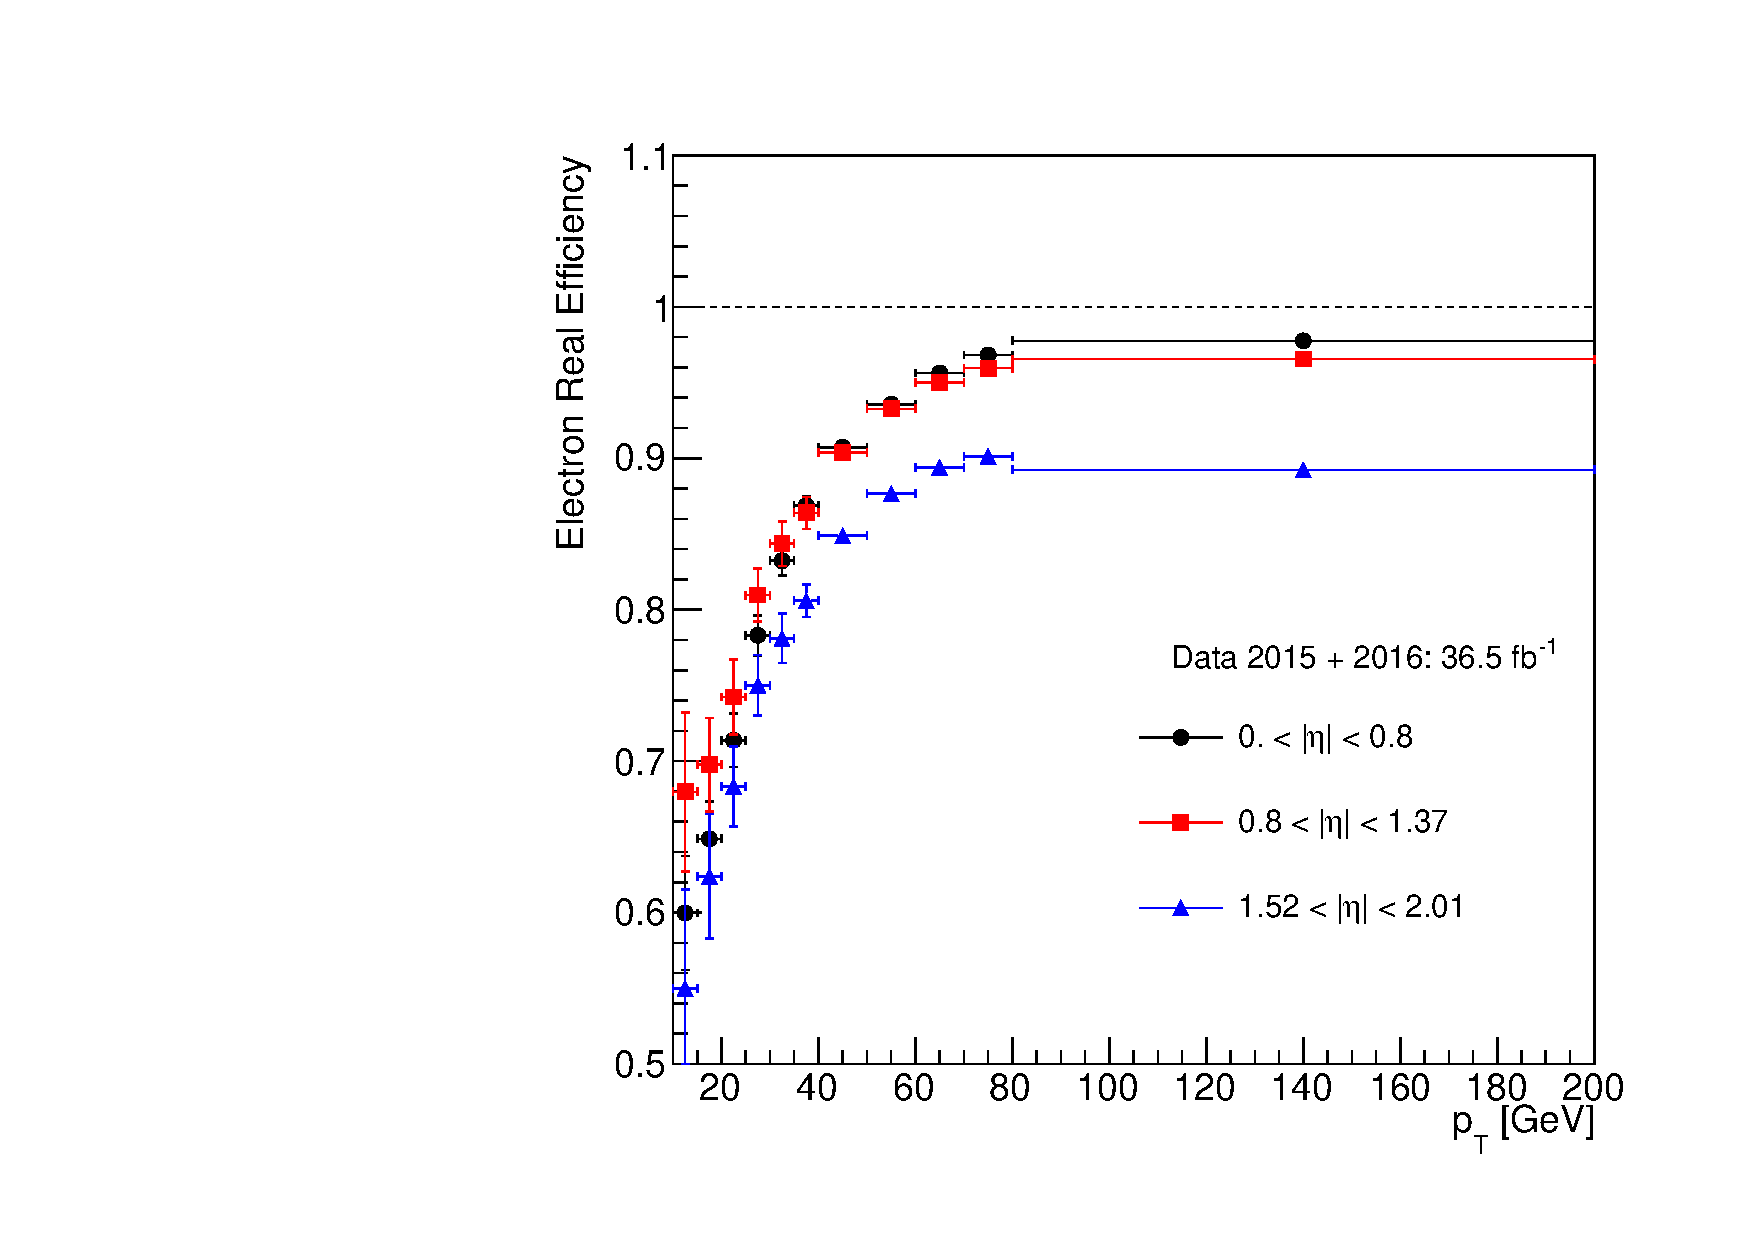
\includegraphics[width=\textwidth]{real_electron_efficiency_total_systematics.pdf}
\subcaption{Electrons}
\end{subfigure}
\begin{subfigure}{0.49\textwidth}
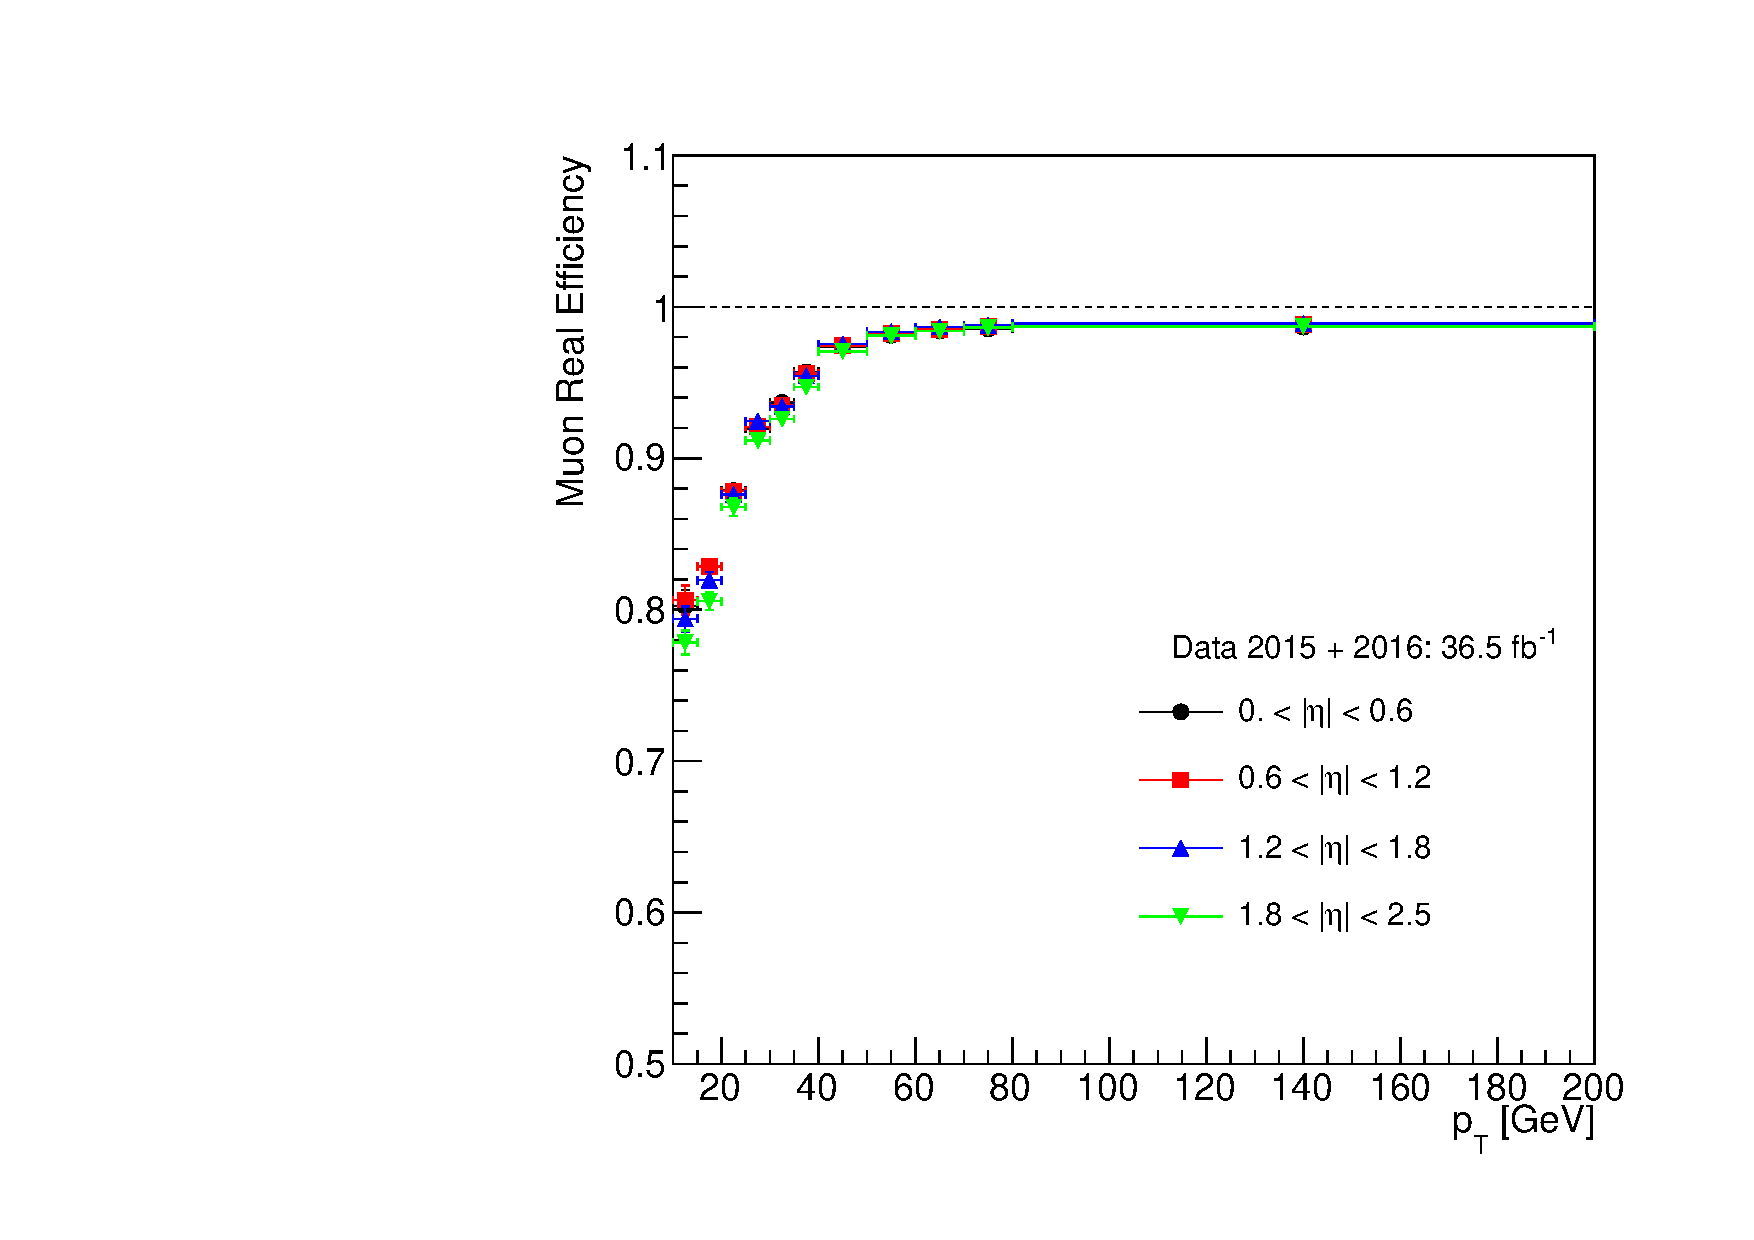
\includegraphics[width=\textwidth]{real_muon_efficiency_total_systematics.pdf}
\subcaption{Muons}
\end{subfigure}
\caption{Baseline-to-signal efficiencies as a function of $\pt$ and $|\eta|$ for real electrons (left) and muons (right), measured in 2015+2016 data.
%The background subtraction is applied on the electron channel only.
The $|\eta|$ binning used in the electron case corresponds to the geometry of the electromagnetic calorimeter.
For muons a homogeneous $|\eta|$ binning is considered.
The error bars corresponds to the quadratic sum of the statistical and tag-and-probe measurement systematic uncertainties.}
\label{fig:prompt_leptons_eff}
\end{figure}

The efficiency is measured as a function of \pt\ and $\eta$, and the results are presented in Figure\ref{fig:prompt_leptons_eff} for electrons and muons. 
The background subtraction is applied on the electron channel only. 
The following systematic uncertainties are assigned to the measured efficiencies: 

\begin{itemize}
\item[$\bullet$] Background contamination: 27 variations of the tag-and-probe method are considered to assess the electron measurement systematics.
Three $m_{ee}$ windows and 9 variations of the background subtraction methods are considered.
The largest contribution to the systematics arises from the $m_{ee}$ window variation.
This is expected as the proportion of electrons affected by Brehmstrahlung depends on $m_{ee}$.
The resulting relative systematics vary from 6\% $\sim$ 12\% in the $10<\pt<15~\GeV$ region, 3\% to 6\% in the $15<\pt<20~\GeV$ region, 1\% to 3\% in the $20<\pt<40~\GeV$ region, and less than 1\% for $\pt >$ 40 \GeV.
The systematic uncertainties associated to the muon efficiencies measurement vary from 1\% to 1.3\% in the $10<\pt<15~\GeV$ region and less than 1\% for $\pt >$ 15 \GeV. 
\item[$\bullet$] Trigger: a systematic uncertainty accounting for a potential bias at trigger level is considered and it varies between 0 and 4\%, depending on the \pt range.
\item[$\bullet$] Extrapolation to busy environments: efficiencies are typically lower in such environments due to the proximity of jets and leptons; 
an uncertainty is assigned by comparing efficiencies in simulated $Z\to\ell\ell$ and $\gluino\to\ttbar\neut$ events, for $\Delta m(\gluino,\neut)>1~\TeV$ which represents an extreme case of final states with highly boosted top quarks. 
The uncertainty, taken as the difference in efficiencies, is parametrized as a function of \pt\ and $\Delta R$ (the angular distance between the lepton and the closest jet). 
\end{itemize}
%The resulting systematic uncertainties are summarized in Table~\ref{tab:RLE_systematics_bkg} and Table~\ref{tab:RLE_systematics_busy}. 
The resulting systematic uncertainties are summarized in Table~\ref{tab:RLE_systematics_all} and Table~\ref{tab:RLE_systematics_busy}.
\begin{center}
\begin{table}
\resizebox{\textwidth}{!}{%
\begin{tabular}{cccc|cccc}
\hline
\hline
& \multicolumn{3}{c}{Electrons} & \multicolumn{3}{c}{Muons}\\
& $0<|\eta|<0.8$ & $0.8<|\eta|<1.37$ & $1.52<|\eta|<2.01$ & $0<|\eta|<0.6$ & $0.6<|\eta|<1.2$ & $1.2<|\eta|<1.8$ & $1.8<|\eta|<2.5$\\
\hline
10~\GeV~$< p_{\text T} <$ 15~\GeV~& 0.047 & 0.063 & 0.089 & 0.014 & 0.010 & 0.008 & 0.011\\
15~\GeV~$< p_{\text T} <$ 20~\GeV~& 0.027 & 0.042 & 0.062 & 0.005 & 0.006 & 0.008 & 0.011\\
20~\GeV~$< p_{\text T} <$ 25~\GeV~& 0.018 & 0.031 & 0.041 & 0.003 & 0.006 & 0.010 & 0.010\\
25~\GeV~$< p_{\text T} <$ 30~\GeV~& 0.029 & 0.024 & 0.027 & 0.011 & 0.015 & 0.022 & 0.019\\
30~\GeV~$< p_{\text T} <$ 35~\GeV~& 0.023 & 0.021 & 0.023 & 0.007 & 0.009 & 0.014 & 0.011\\
35~\GeV~$< p_{\text T} <$ 40~\GeV~& 0.014 & 0.018 & 0.018 & 0.004 & 0.004 & 0.006 & 0.006\\
40~\GeV~$< p_{\text T} <$ 50~\GeV~& 0.007 & 0.010 & 0.010 & 0.002 & 0.001 & 0.002 & 0.001\\
50~\GeV~$< p_{\text T} <$ 60~\GeV~& 0.008 & 0.010 & 0.010 & 0.001 & 0.001 & 0.001 & 0.001\\
60~\GeV~$< p_{\text T} <$ 70~\GeV~& 0.007 & 0.010 & 0.010 & 0.001 & 0.001 & 0.001 & 0.002\\
70~\GeV~$< p_{\text T} <$ 80~\GeV~& 0.008 & 0.011 & 0.012 & 0.002 & 0.001 & 0.001 & 0.002\\
80~\GeV~$< p_{\text T} <$ 120~\GeV~& 0.010 & 0.010 & 0.011 & 0.004 & 0.002 & 0.002 & 0.002\\
120~\GeV~$< p_{\text T} <$ 150~\GeV~& 0.005 & 0.005 & 0.011 & 0.006 & 0.005 & 0.005 & 0.005\\
150~\GeV~$< p_{\text T} <$ 200~\GeV~& 0.005 & 0.002 & 0.019 & 0.005 & 0.005 & 0.005 & 0.006\\
\hline
\hline
\end{tabular}
}
\caption{
Systematic uncertainties on the measured real lepton efficiency, separating sources affecting the measurement itself (background subtraction, trigger bias, and different methods). 
}
\label{tab:RLE_systematics_all}
\end{table}
\end{center}

\begin{center}
\begin{table}
\resizebox{\textwidth}{!}{%
\begin{tabular}{ccccccccccc}
\hline
\hline
\multicolumn{9}{c}{electrons (busy environments)}\\
\hline
$\Delta R(e, jet)$ & [0, 0.1] & [0.1, 0.15] & [0.15, 0.2] & [0.2, 0.3] & [0.3, 0.35] & [0.35, 0.4] & [0.4, 0.6] & [0.6, 4]\\
\hline
10~\GeV~$< p_{\text T} <$ 20~\GeV~& - & - & - & - & - & - & 25.31\% & 6.5\%\\
20~\GeV~$< p_{\text T} <$ 30~\GeV~& - & - & - & - & - & 73.37\% & 10.21\% & 0.37\%\\
30~\GeV~$< p_{\text T} <$ 40~\GeV~& - & - & - & 97.71\% & 48.22\% & 15.54\% & 7.29\% & 0.58\%\\
40~\GeV~$< p_{\text T} <$ 50~\GeV~& - & - & - & 52.81\% & 22.80\% & 16.73\% & 7.68\% & 1.10\%\\
50~\GeV~$< p_{\text T} <$ 60~\GeV~& - & - & - & 29.96\% & 21.49\% & 20.23\% & 6.99\% & 2.78\%\\
60~\GeV~$< p_{\text T} <$ 80~\GeV~& - & - & 55.89\% & 24.31\% & 17.40\% & 24.77\% & 6.20\% & 2.87\%\\
80~\GeV~$< p_{\text T} <$ 150~\GeV~& - & 57.52\% & 30.24\% & 16.45\% & 12.73\% & 20.92\% & 4.44\% & 2.73\%\\
150~\GeV~$< p_{\text T} <$ 200~\GeV~& 88.54\% & 40.16\% & 19.34\% & 8.45\% & 14.66\% & 16.57\% & 2.57\% & 1.90\%\\
\hline
\hline
%\end{tabular}
%}
%\resizebox{\textwidth}{!}{%
%\begin{tabular}{ccccccccccc}
%\hline
%\hline
\multicolumn{9}{c}{muons (busy environments)}\\
\hline
$\Delta R(\mu, jet)$ & [0, 0.1] & [0.1, 0.15] & [0.15, 0.2] & [0.2, 0.3] & [0.3, 0.35] & [0.35, 0.4] & [0.4, 0.6] & [0.6, 4]\\
\hline
10~\GeV~$< p_{\text T} <$ 20~\GeV~& - & - & - & - & - & - & 33.59\% & 5.18\%\\
20~\GeV~$< p_{\text T} <$ 30~\GeV~& - & - & - & - & - & 82.34\% & 22.27\% & 3.39\%\\
30~\GeV~$< p_{\text T} <$ 40~\GeV~& - & - & -  & 98.54\% & 56.36\% & 31.89\% & 14.22\% & 2.24\%\\
40~\GeV~$< p_{\text T} <$ 50~\GeV~& - & - & - & 53.10\% & 21.33\% & 13.90\% & 6.81\% & 1.45\%\\
50~\GeV~$< p_{\text T} <$ 60~\GeV~& - & - & - & 24.98\% & 13.72\% & 9.62\% & 3.83\% & 0.79\%\\
60~\GeV~$< p_{\text T} <$ 80~\GeV~& - & - & 44.41\% & 13.75\% & 6.14\% & 4.76\% & 2.04\% & 0.15\%\\
80~\GeV~$< p_{\text T} <$ 150~\GeV~& - & 29.94\% & 7.14\% & 3.16\% & 1.30\% & 1.04\% & 0.07\% & 0.57\%\\
150~\GeV~$< p_{\text T} <$ 200~\GeV~& 82.26\% & 4.14\% & 1.02\% & 0.17\% & 0.29\% & 0.62\% & 1.02\% & 1.13\%\\
\hline
\hline
\end{tabular}
}
\caption{
Systematic uncertainties on the measured real lepton efficiency, due to the extrapolation to busy environments using $\gluino \to \ttbar \tilde{\chi_1^0}$ events. 
}
\label{tab:RLE_systematics_busy}
\end{table}
\end{center}
